\section{Results}
\label{sec:results}

We present results in mechanism-first order (E6/E2 lead; E1/E12 confirm aggregate
behaviour), matching Chapter~\ref{ch:results}.
Canonical numbers use \texttt{run\_e1\_canonical\_v1} and
\texttt{run\_e12\_canonical\_v1} on current BENCH-120 (fingerprint
\texttt{322157816b37c34e}).

%% -------------------------------------------------------------------
\subsection{RQ4: Specification Complexity Scaling (E3)}
%% -------------------------------------------------------------------

\begin{figure}[t]
  \centering
  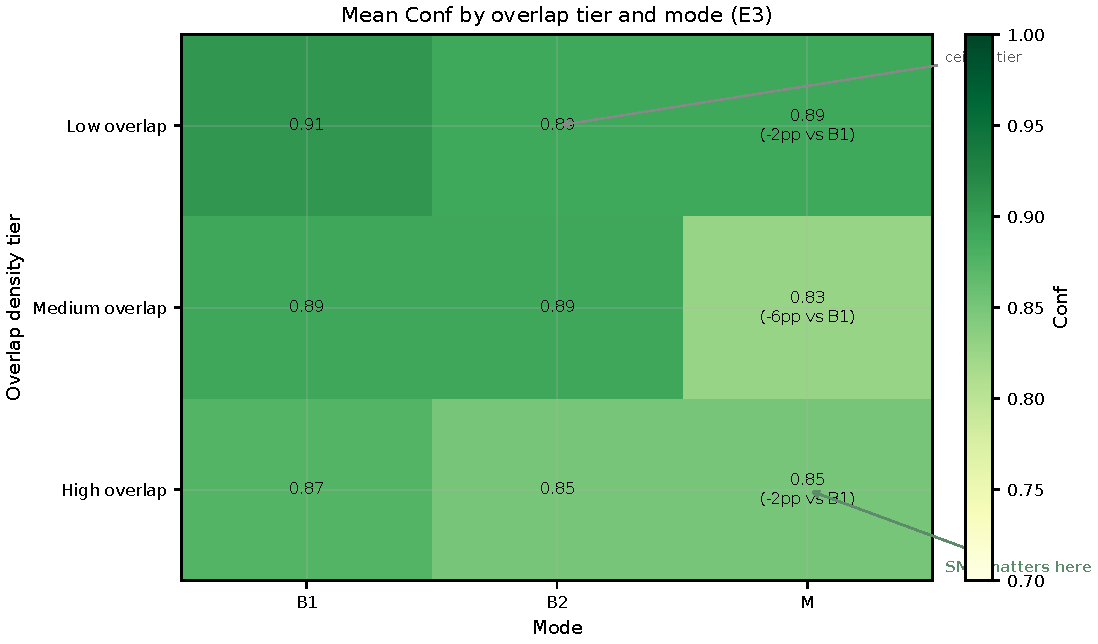
\includegraphics[width=\linewidth]{figures/complexity_heatmap.pdf}
  \caption{Mean strict formal conformance by overlap-density tier and mode.
    Tertiles on canonical E1 are \emph{not} monotone for M vs.\ B2; deployment
    should follow Table~\ref{tab:deployment-boundary}, not a single overlap rule.}
  \label{fig:complexity}
\end{figure}

Figure~\ref{fig:complexity} stratifies the 120-task benchmark by overlap-density tertile.
In the \textbf{low} tier ($n{=}49$), B1 leads (91.9\%); M ties B2 (89.9\%).
In the \textbf{medium} tier ($n{=}33$), B1/B2 tie (87.5\%); M trails (82.2\%).
In the \textbf{high} tier ($n{=}38$), B1 leads (87.4\%); M ties B2 (85.1\%).
E10 on 100 unfiltered random tasks confirms the same pattern: B2 leads aggregate
conformance (89.1\% vs.\ M 83.1\%, 0/100 wins).

\paragraph{Answer to RQ4.}
Overlap tertiles bound C1 but do not justify universal M $>$ B2.
The controlled E6 comparison (+7.7\,pp typed feedback) and E12 multi-seed ranking
(B2 leads all seeds) are the primary mechanism and stability evidence.

%% -------------------------------------------------------------------
\subsection{RQ3: Component Attribution (E5, E6, Ablation)}
%% -------------------------------------------------------------------

\paragraph{Repair dynamics (E5).}

\begin{figure}[t]
  \centering
  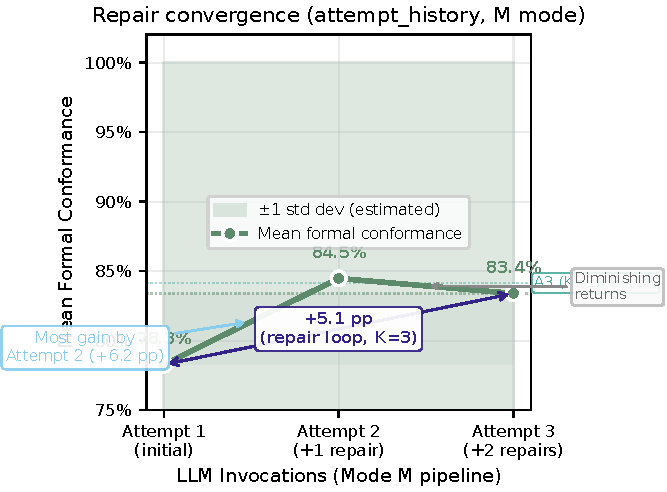
\includegraphics[width=\linewidth]{figures/repair_convergence.pdf}
  \caption{Mean strict formal conformance at each repair iteration for M (Semantic
    Feedback IR) vs.\ B2 (test-only feedback).  Most M gain arrives by
    iteration~2.  Shaded bands are 95\% bootstrap confidence intervals.}
  \label{fig:convergence}
\end{figure}

Figure~\ref{fig:convergence} shows the $\mathrm{Conf}(k)$ trajectory extracted from
\texttt{attempt\_history} logs.
Mode~M rises from 78.3\% at $k{=}1$ to 84.5\% at $k{=}2$, then plateaus at 83.4\%
at $k{=}3$---justifying budget $K{=}3$ without claiming monotone dominance over B2.

\paragraph{Feedback variant isolation (E6).}

\begin{figure}[t]
  \centering
  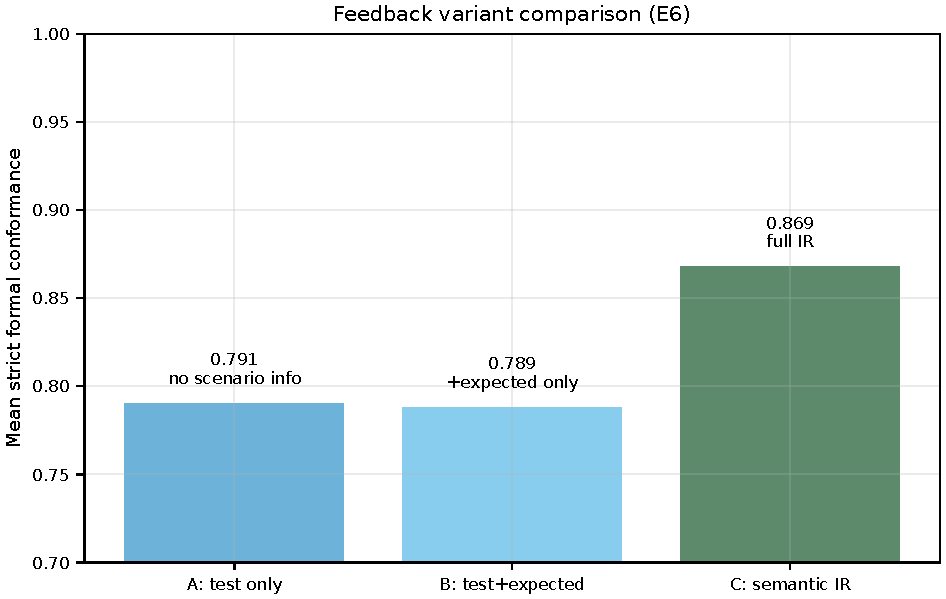
\includegraphics[width=\linewidth]{figures/feedback_variant_bar.pdf}
  \caption{Final Conf and mean iterations-to-convergence for feedback variants
    A (test only), B (test + expected), and C (full Semantic Feedback IR).
    Progressive improvement from A to C confirms that specification-level structure,
    not prompt volume, drives the repair benefit.}
  \label{fig:feedback-variant}
\end{figure}

Figure~\ref{fig:feedback-variant} shows Conf(C) $>$ Conf(B) $\approx$ Conf(A)
(86.9\%, 78.9\%, 79.1\%).
Variant~C improves mean conformance by \textbf{+7.7\,pp} over test-only feedback---the
paper's lead empirical claim.
Mean iterations are nearly identical ($\approx$2.98 across variants).

\paragraph{Ablation (E1/RQ3).}

\begin{figure}[t]
  \centering
  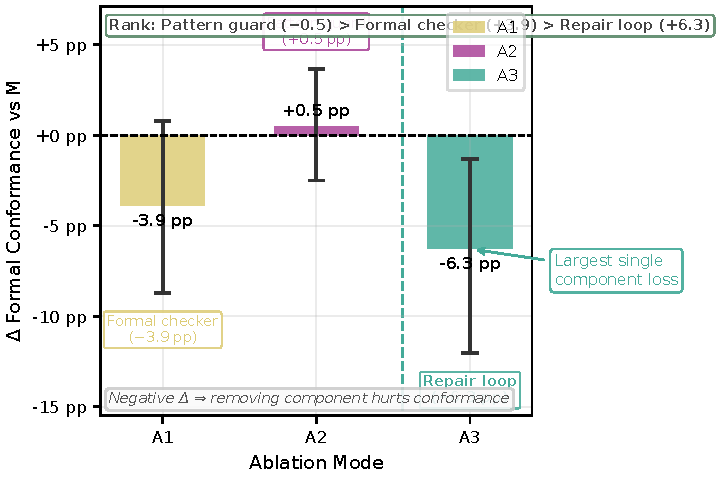
\includegraphics[width=\linewidth]{figures/ablation_contribution_ci.pdf}
  \caption{Ablation deltas relative to full M.  Error bars show 95\% bootstrap
    confidence intervals.  By $|\Delta\mathrm{Conf}|$: A2 ($-$6.0\,pp) $>$
    A3 ($-$3.9\,pp) $>$ A1 ($-$0.8\,pp).}
  \label{fig:ablation}
\end{figure}

Table~\ref{tab:main} and Figure~\ref{fig:ablation} show component attributions on
canonical E1.
Removing the pattern guard (A2) causes the largest conformance drop
($\Delta = -6.0$\,pp; 80.3\% vs.\ M 86.3\%)---A2 does \emph{not} beat M.
Removing the repair loop (A3) costs $-$3.9\,pp; removing the formal checker
(A1) costs $-$0.8\,pp.
Ranking by $|\Delta\mathrm{Conf}|$: A2 $>$ A3 $>$ A1.
The guard's prevention value is additionally measured via PDR/FAR (E2).

\paragraph{Answer to RQ3.}
On Conf.\ ablations, pattern-guard removal (A2) dominates, then repair (A3),
then the formal checker (A1).
Semantic Feedback IR (E5/E6) remains the lead mechanism claim for typed repair;
the pattern guard is also a prevention/diagnostic gate (E2 PDR/FAR).

%% -------------------------------------------------------------------
\subsection{RQ1: Overall Effectiveness (E1)}
%% -------------------------------------------------------------------

\begin{table}[t]
  \caption{Main results on BENCH-120 (\texttt{run\_e1\_canonical\_v1}, repeat~0).
    E12-canonical is authoritative for B1/B2/M ranking across seeds.}
  \label{tab:main}
  \centering
  \small
  \begin{tabular}{lrrrrrr}
    \toprule
    Mode & Strict\% & Conf\% & Kill\% & PDR\% & FAR\% & Latency (s) \\
    \midrule
    B0 & 5.0 & 89.2 & 48.6 & --- & --- & 0.2 \\
    B1 & 5.0 & 89.2 & 48.6 & 43.0 & 56.6 & 11.7 \\
    B2 & 5.0 & 87.7 & 48.9 & 88.4 & 11.5 & 13.9 \\
    B3 & 5.0 & 81.9 & 51.0 & --- & --- & 13.2 \\
    B4 & 5.0 & 87.1 & 49.3 & --- & --- & 10.8 \\
    M  & 5.0 & 86.3 & 49.8 & 90.3 & 9.6 & 46.2 \\
    A1 & 5.0 & 85.5 & 49.5 & 90.4 & 9.6 & 58.6 \\
    A2 & 5.0 & 80.3 & 50.9 & 88.1 & 11.9 & 39.9 \\
    A3 & 3.3 & 82.4 & 51.0 & 90.6 & 9.4 & 6.6 \\
    \bottomrule
  \end{tabular}
\end{table}

Canonical E1 at seed~0: B1 89.2\%, B2 87.7\%, M 86.3\% (Table~\ref{tab:main}; all
Holm n.s.).
E12-canonical ($120{\times}3$ seeds): B2 leads every seed (88.0\% mean vs.\ M 86.0\%);
M wins 4/120 paired comparisons; Friedman $p{=}0.077$.

\paragraph{The strict-success paradox.}
On current BENCH-120, strict success is uniformly low (5.0\% across B1/B2/M) because
conjunctive $\mathrm{Accept}$ is selective by design.
Prevention metrics (PDR/FAR) differentiate M from B2; see E2.

\paragraph{Answer to RQ1.}
B1 leads mean strict formal conformance at 89.2\% on canonical E1; M reaches
86.3\%.
Conformance, not strict success, is the appropriate discriminating metric on hard
precedence-sensitive benchmarks.

%% -------------------------------------------------------------------
\subsection{RQ2: Fault Class Prevention (E2, E7)}
%% -------------------------------------------------------------------

\begin{figure}[t]
  \centering
  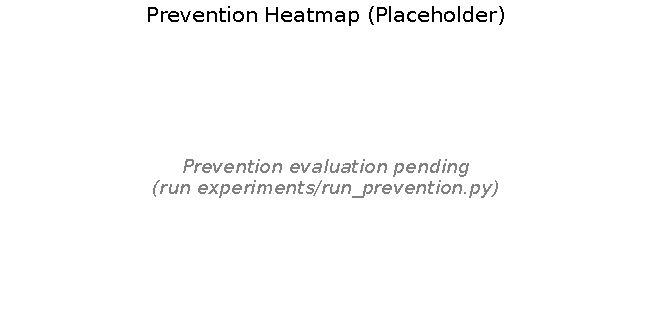
\includegraphics[width=\linewidth]{figures/prevention_heatmap_by_mode_eval.pdf}
  \caption{PDR heatmap by mode (rows) and evaluation type (columns).  M leads on
    implementation screening; modes are complementary across fault families.}
  \label{fig:prevention-heatmap}
\end{figure}

\begin{figure}[t]
  \centering
  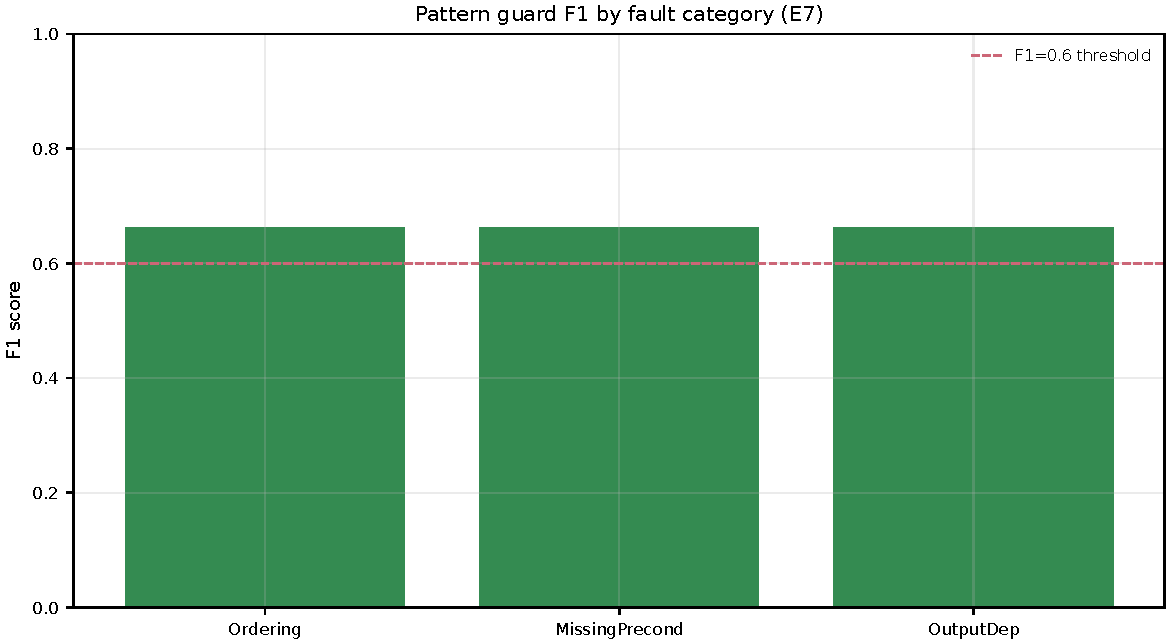
\includegraphics[width=\linewidth]{figures/pattern_guard_f1_bar.pdf}
  \caption{Pattern guard precision, recall, and F1 per fault category on the E2
    mutant population.  Ordering categories achieve F1 $\approx$0.67, consistent with
    the guard's design targeting FSF scenario-order violations.}
  \label{fig:pattern-f1}
\end{figure}

Figure~\ref{fig:prevention-heatmap} reveals complementary prevention: no single mode
wins every column, but M leads on specification-structural faults while B2 remains
competitive on boundary-shift operators.
Aggregate PDR/FAR on the full E2 population ($n{=}1{,}704$ evaluations per mode):
M 95.0\%/5.0\% vs.\ B2 91.2\%/8.8\%.

Figure~\ref{fig:pattern-f1} shows per-category F1 for the pattern guard.
Ordering categories reach F1 $\approx$0.67, confirming the guard functions as a
specification-derived defect classifier rather than a heuristic rule set.

\paragraph{Answer to RQ2.}
The framework prevents ordering and guard-inversion defects most effectively.
Boundary-shift defects are better detected by test-feedback baselines.
Deploy full M when PDR/FAR and conjunctive Accept matter; otherwise prefer B2
(Table~\ref{tab:deployment-boundary}).

%% -------------------------------------------------------------------
\subsection{RQ5: Quality--Overhead Trade-off (E1)}
%% -------------------------------------------------------------------

\begin{figure}[t]
  \centering
  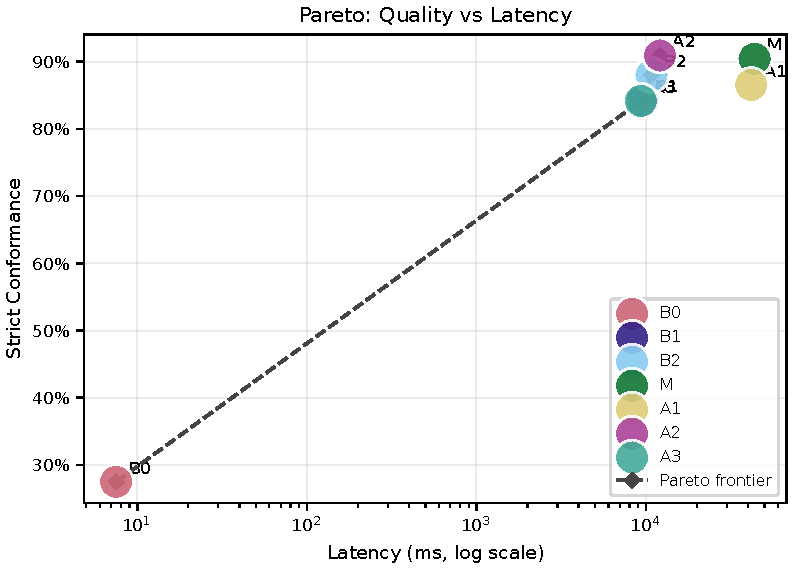
\includegraphics[width=\linewidth]{figures/pareto_quality_vs_latency.pdf}
  \caption{Pareto view of strict formal conformance vs.\ mean latency per task.
    B2 is the default latency--quality point; M trades $3.3\times$ latency for
    best prevention (PDR/FAR).}
  \label{fig:pareto}
\end{figure}

Figure~\ref{fig:pareto} shows B2 at 13.9\,s and 87.7\% Conf.\ as the practical default.
M pays $3.3\times$ latency (46.2\,s vs.\ 13.9\,s) for higher prevention, not higher
mean Conf.\ on canonical E1.
A2 (39.9\,s, 80.3\% Conf.) is a lower-prevention ablation point, not a Conf.\ upgrade
over M.

\paragraph{Answer to RQ5.}
Default to B2 for mean conformance and latency; deploy M when conjunctive Accept,
PDR/FAR, or E6-typed feedback justify the overhead.

%% -------------------------------------------------------------------
\subsection{RQ4 Extended: Boundary Density (E4)}
%% -------------------------------------------------------------------

\begin{figure}[t]
  \centering
  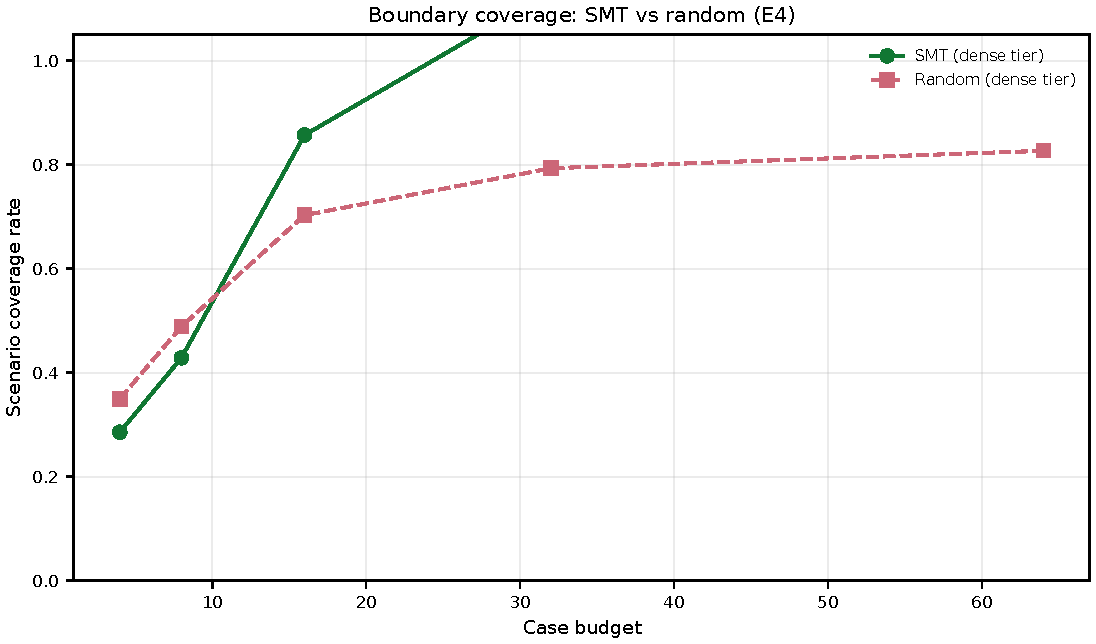
\includegraphics[width=\linewidth]{figures/boundary_coverage_by_density.pdf}
  \caption{Scenario coverage rate vs.\ case budget for SMT witnesses and random
    sampling, stratified by overlap density.  Random sampling degrades in the
    high-density tier; SMT maintains higher coverage at equal budget.}
  \label{fig:boundary}
\end{figure}

Figure~\ref{fig:boundary} shows that at budget~16, random sampling covers
$\approx$70\% of the high-density tier vs.\ $\approx$86\% for SMT-guided witnesses.
The gap shrinks in sparse tiers, explaining why test-feedback baselines perform
adequately on simple specifications but degrade on hard ones.

%% -------------------------------------------------------------------
\subsection{Generalisation Study (E8)}
%% -------------------------------------------------------------------

\begin{figure}[t]
  \centering
  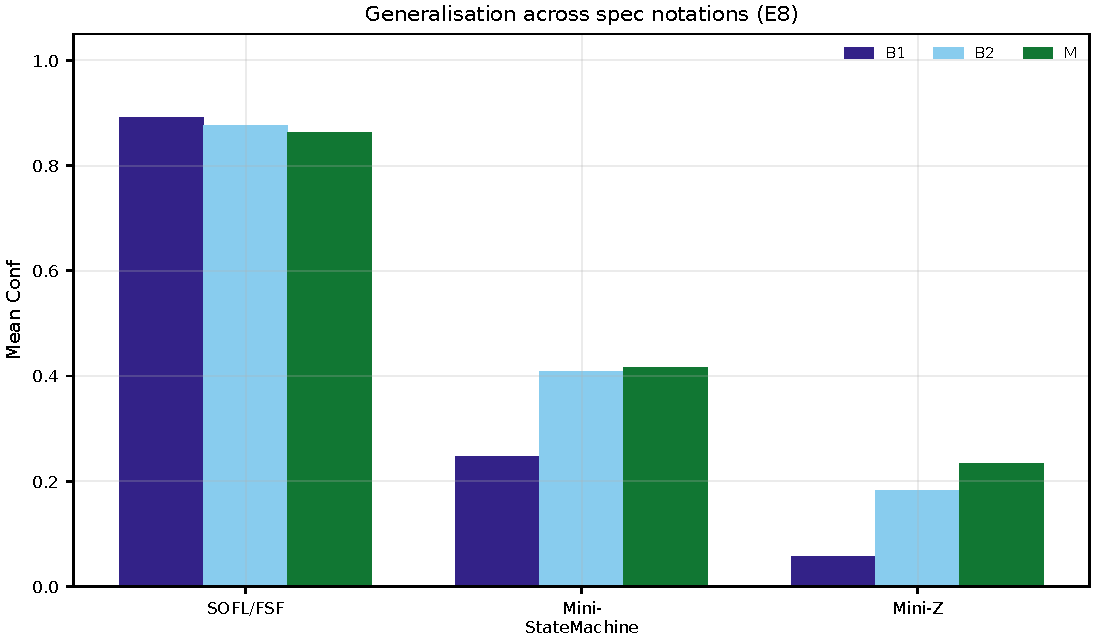
\includegraphics[width=\linewidth]{figures/generalisation_bar.pdf}
  \caption{Strict formal conformance across specification notations.  Gains are
    notation-dependent; SOFL/FSF and real-derived subsets do not uniformly favour M.}
  \label{fig:generalisation}
\end{figure}

Table~\ref{tab:generalisation} and Figure~\ref{fig:generalisation} show M vs.\ B1/B2
across notation adapters and real-derived subsets.
M beats B1 on Mini adapters; on SOFL/FSF canonical E1, B1/B2 lead M on aggregate
conformance; HumanEval-FSF favours B2 (98.8\% vs.\ M 87.1\%).
We report boundary cases transparently and scope deployment claims to
Table~\ref{tab:deployment-boundary}.

\begin{table}[t]
  \caption{Generalisation results: Conf by specification notation and mode.}
  \label{tab:generalisation}
  \centering
  \small
  \begin{tabular}{lccc}
    \toprule
    Notation & B1 Conf\% & B2 Conf\% & M Conf\% \\
    \midrule
    SOFL/FSF (120 tasks) & 89.2 & 87.7 & 86.3 \\
    Mini-StateMachine (30 tasks) & 24.7 & 40.8 & 41.6 \\
    Mini-Z (30 tasks) & 5.8 & 18.3 & 23.3 \\
    HumanEval-FSF (20 tasks) & 89.7 & 98.8 & 87.1 \\
    MBPP-FSF (20 tasks) & 90.0 & 95.0 & 95.0 \\
    \bottomrule
  \end{tabular}
\end{table}

\begin{table}[t]
\caption{Statistical test summary for E1 (120-task hard benchmark, repeat~0). Wilcoxon signed-rank for per-task strict success and conformance; Mann--Whitney~U for latency. Holm--Bonferroni correction within each metric family. Cliff's $\delta$: positive favours the first mode in each pair.}
\label{tab:stats}
\centering
\small
\begin{tabular}{lccc}
\toprule
Comparison & $p$ (Holm) & Significant ($\alpha{=}0.05$) & Cliff's $\delta$ / ratio \\
\midrule
\multicolumn{4}{l}{\textit{Primary comparisons}} \\
\addlinespace
\texttt{M} vs \texttt{B1} (strict success) & 1.0000 & No & -0.0167 \\
\texttt{M} vs \texttt{B2} (strict success) & 1.0000 & No & -0.0167 \\
\texttt{M} vs \texttt{B1} (conformance) & 0.0745 & No & +0.0358 \\
\texttt{M} vs \texttt{B2} (conformance) & 0.8113 & No & +0.0002 \\
\texttt{M} vs \texttt{B2} (latency) & <0.001 & Yes & 4.05$\times$ \\
\addlinespace
\multicolumn{4}{l}{\textit{All pairwise conformance (Holm-corrected)}} \\
\addlinespace
\texttt{A1} vs \texttt{B0} (Conf) & <0.001 & Yes & +0.4750 \\
\texttt{A1} vs \texttt{B1} (Conf) & 1.0000 & No & +0.0227 \\
\texttt{A1} vs \texttt{B2} (Conf) & 1.0000 & No & -0.0112 \\
\texttt{A1} vs \texttt{M} (Conf) & 1.0000 & No & -0.0119 \\
\texttt{A2} vs \texttt{A1} (Conf) & 0.9931 & No & +0.0285 \\
\texttt{A2} vs \texttt{B0} (Conf) & <0.001 & Yes & +0.5112 \\
\texttt{A2} vs \texttt{B1} (Conf) & 0.0745 & No & +0.0517 \\
\texttt{A2} vs \texttt{B2} (Conf) & 1.0000 & No & +0.0171 \\
\texttt{A2} vs \texttt{M} (Conf) & 1.0000 & No & +0.0174 \\
\texttt{A3} vs \texttt{A1} (Conf) & 1.0000 & No & -0.0272 \\
\texttt{A3} vs \texttt{A2} (Conf) & 1.0000 & No & -0.0568 \\
\texttt{A3} vs \texttt{B0} (Conf) & <0.001 & Yes & +0.4569 \\
\texttt{A3} vs \texttt{B1} (Conf) & 1.0000 & No & -0.0044 \\
\texttt{A3} vs \texttt{B2} (Conf) & 1.0000 & No & -0.0387 \\
\texttt{A3} vs \texttt{M} (Conf) & 1.0000 & No & -0.0407 \\
\texttt{B1} vs \texttt{B0} (Conf) & <0.001 & Yes & +0.4569 \\
\texttt{B2} vs \texttt{B0} (Conf) & <0.001 & Yes & +0.4871 \\
\texttt{B2} vs \texttt{B1} (Conf) & 1.0000 & No & +0.0341 \\
\texttt{M} vs \texttt{B0} (Conf) & <0.001 & Yes & +0.5067 \\
\texttt{M} vs \texttt{B1} (Conf) & 0.0745 & No & +0.0358 \\
\texttt{M} vs \texttt{B2} (Conf) & 0.8113 & No & +0.0002 \\
\addlinespace
\multicolumn{4}{l}{\textit{All pairwise strict success (Holm-corrected)}} \\
\addlinespace
\texttt{A1} vs \texttt{B0} (strict) & 1.0000 & No & -0.0083 \\
\texttt{A1} vs \texttt{B1} (strict) & 1.0000 & No & +0.0000 \\
\texttt{A1} vs \texttt{B2} (strict) & 1.0000 & No & +0.0000 \\
\texttt{A1} vs \texttt{M} (strict) & 1.0000 & No & +0.0167 \\
\texttt{A2} vs \texttt{A1} (strict) & 1.0000 & No & +0.0000 \\
\texttt{A2} vs \texttt{B0} (strict) & 1.0000 & No & -0.0083 \\
\texttt{A2} vs \texttt{B1} (strict) & 1.0000 & No & +0.0000 \\
\texttt{A2} vs \texttt{B2} (strict) & 1.0000 & No & +0.0000 \\
\texttt{A2} vs \texttt{M} (strict) & 1.0000 & No & +0.0167 \\
\texttt{A3} vs \texttt{A1} (strict) & 1.0000 & No & +0.0000 \\
\texttt{A3} vs \texttt{A2} (strict) & 1.0000 & No & +0.0000 \\
\texttt{A3} vs \texttt{B0} (strict) & 1.0000 & No & -0.0083 \\
\texttt{A3} vs \texttt{B1} (strict) & 1.0000 & No & +0.0000 \\
\texttt{A3} vs \texttt{B2} (strict) & 1.0000 & No & +0.0000 \\
\texttt{A3} vs \texttt{M} (strict) & 1.0000 & No & +0.0167 \\
\texttt{B1} vs \texttt{B0} (strict) & 1.0000 & No & -0.0083 \\
\texttt{B2} vs \texttt{B0} (strict) & 1.0000 & No & -0.0083 \\
\texttt{B2} vs \texttt{B1} (strict) & 1.0000 & No & +0.0000 \\
\texttt{M} vs \texttt{B0} (strict) & 1.0000 & No & -0.0250 \\
\texttt{M} vs \texttt{B1} (strict) & 1.0000 & No & -0.0167 \\
\texttt{M} vs \texttt{B2} (strict) & 1.0000 & No & -0.0167 \\
\bottomrule
\end{tabular}
\end{table}

